\chapter*{Results}

To begin with, spectra with two positron lifetimes, $\tau_1$ and $\tau_2$ were simulated with PALSSIM, using an instrument resolution function (IRF) made up of three gaussians (see Table \ref{tab:irf}). With $\tau_1$ kept fixed at 180ps, spectra were generated for $\tau_2$  = 220-280ps at 10ps intervals using PALSSIM. For each value of $\tau_2$, three spectra were generated, with intensities of $\tau_1$ and $\tau_2$ (respectively) set to 20\%-80\%, 50\%-50\%, 80\%-20\%. The goal was to evaluate how good PALSFIT is at extracting the lifetimes $\tau_1$, $\tau_2$ and their respective intensities, for each simulated spectrum. 

\begin{table}[h]
    \centering
    \begin{tabular}{|c|c|c|}
        \hline
        FWHM (ps) &  Shift (ps) & Intensity (\%) \\
        \hline
        213.3 & 0 & 80\\ 
        150 & -5 & 10\\ 
        267 & 17 & 10\\  
        \hline
    \end{tabular}
    \caption{Instrument resolution function}
    \label{tab:irf}
\end{table}

Starting with $\tau_1$, we can see in Figure \ref{fig:180-tau1} that for some values of $\tau_2$ the software performed well at fitting the shorter lifetime, while it struggled for others. 
Zooming in specifically to the $\tau_2$ = 250-270ps range, we can see in Figure \ref{fig:180-tau1-zoomed} that, for these values in particular, it struggled to determine $\tau_1$ in the 50-50 and 80-20 case. 

\begin{figure}
    \centering
    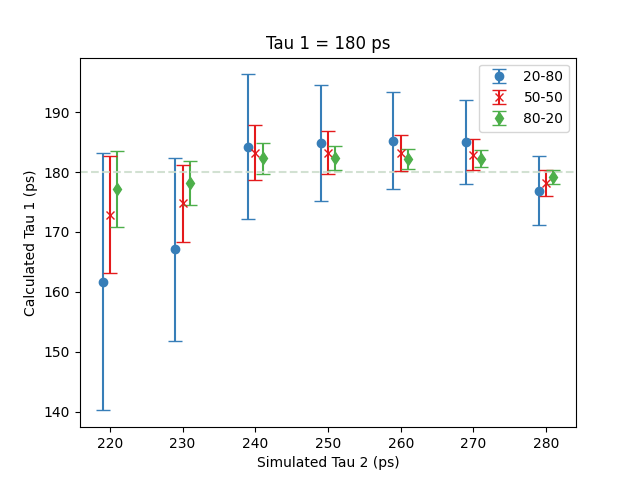
\includegraphics[width=0.8\linewidth]{Batch 1+2/Tau1.png}
    \caption{fixed $\tau_1 = 180ps$}
    \label{fig:180-tau1}
\end{figure}

\begin{figure}
    \centering
    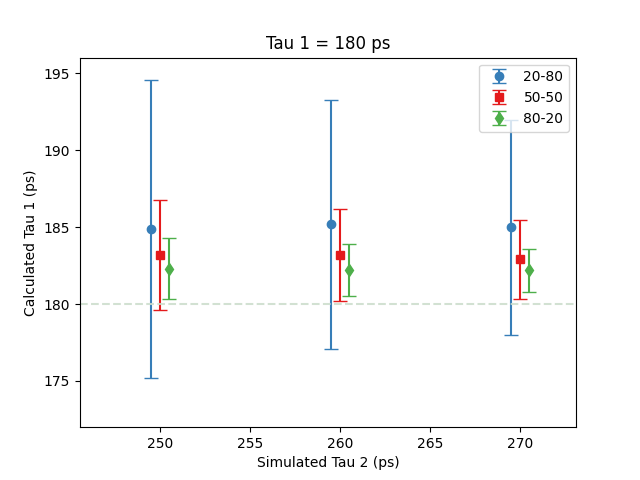
\includegraphics[width=0.8\linewidth]{Batch 1+2/Tau1 stragglers.png}
    \caption{close-up $\tau_1 = 180ps$}
    \label{fig:180-tau1-zoomed}
\end{figure}

\begin{figure}
    \centering
    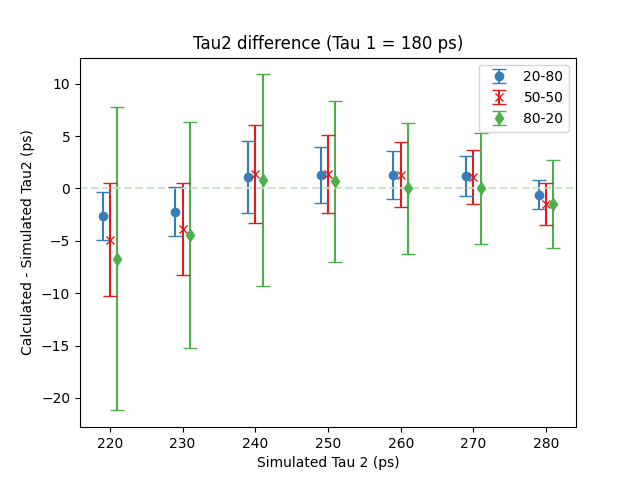
\includegraphics[width=0.8\linewidth]{Batch 1+2/Tau2 diff.png}
    \caption{$\tau_2$ difference}
    \label{fig:180-tau2}
\end{figure}

To evaluate how the software performs in detecting $\tau_2$, we do the same as before, but instead of plotting $\tau_1$ on the y axis, we can plot the difference between the result and the original simulated values of $\tau_2$ to essentially tells us how far off PALSFIT is from the simulated value. Doing so we can see in Figure \ref{fig:180-tau2} that, aside from the 20-80 spectrum for $\tau_2$ = 220, here PALSFIT performs reasonably well.

Observing the error bars in the figures lets us know how confident our fit for the two lifetimes is. From here we can notice two important factors that affect the precision of the fitting. By looking at Figure \ref{fig:180-tau1} and Figure \ref{fig:180-tau2}, we can deduce that the relative intensities of the two lifetimes is one of them. In Figure \ref{fig:180-tau1}, where we are analysing $\tau_1$, the error bars are the smallest for the 80-20 data, where the shorter lifetime is more intense, and in Figure 3, the opposite is the case and we have the 20-80 data being the most precise. Looking at all the figures, we can also notice that the error bars progressively shrink as the time interval between the lifetimes, which is the second factor, increases. Both these facts make intuitive sense.

\begin{figure}
    \centering
    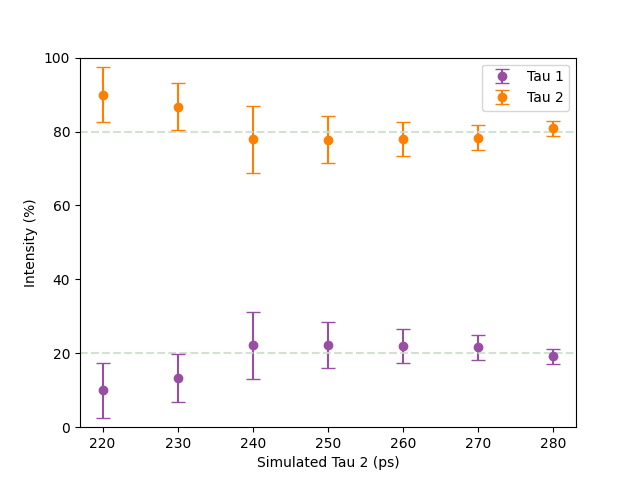
\includegraphics[width=0.8\linewidth]{Batch 1+2/2080.png}
    \caption{$\tau_1 = 20\%, \tau_1 = 80\%$}
    \label{fig:180-2080}
\end{figure}

\begin{figure}
    \centering
    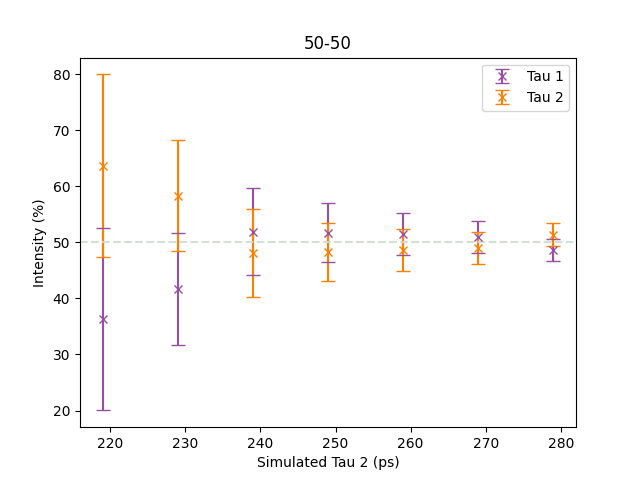
\includegraphics[width=0.8\linewidth]{Batch 1+2/5050.png}
    \caption{$\tau_1 = 50\%, \tau_1 = 50\%$}
    \label{fig:180-5050}
\end{figure}

\begin{figure}
    \centering
    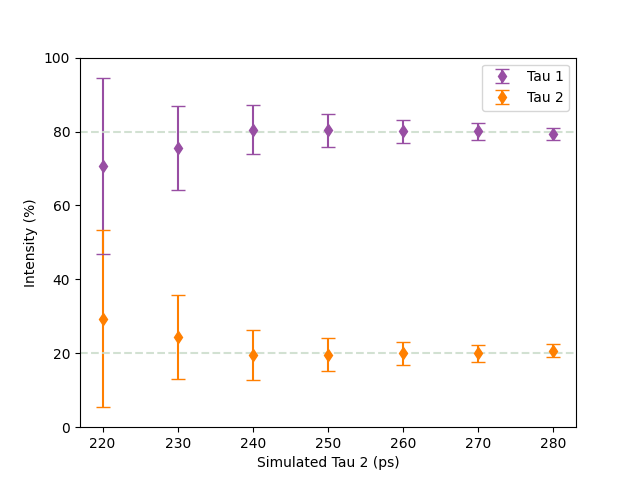
\includegraphics[width=0.8\linewidth]{Batch 1+2/8020.png}
    \caption{$\tau_1 = 80\%, \tau_1 = 20\%$}
    \label{fig:180-8020}
\end{figure}

In Figure \ref{fig:180-2080} - Figure \ref{fig:180-8020}, we can observe that when the relative intensity of $\tau_2$ was greater or equal to $\tau_1$, then PALSFIT was able to calculate the appropriate lifetime intensities. However, when the intensity of $\tau_2$ was at 80\%, as we can see in Figure \ref{fig:180-2080}, for the first two simulated values of $\tau_2$, the software was unable to output the correct intensities. Looking at our error bars, we can see the same relationship between the size of the error bars and the time separation of the two lifetimes.

On the whole then, PALSFIT seemed to perform reasonably well, but not perfectly. As the first lifetime, $\tau_1$, was kept constant at 180ps, the next step would be to change $\tau_1$ and see how that might alter our results. We can bring down $\tau_1$ to 150 and perform the same analysis.  To keep things consistent, we’ll modify our $\tau_2$ range to maintain the spacing between the lifetimes consistent between runs. As such, we’ll set $\tau_2$ = 180-250ps . The results are in the figures below.

\begin{figure}
    \centering
    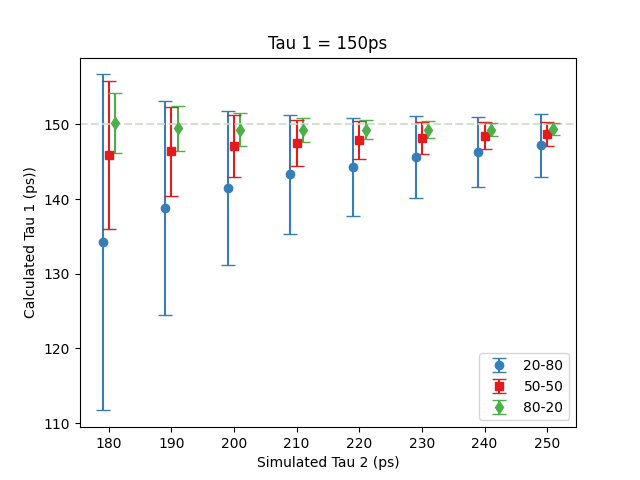
\includegraphics[width=0.8\linewidth]{Batch 3/regular IRF/tau1 150/output/t1.png}
    \caption{fixed $\tau_1 = 150ps$}
    \label{fig:150-8020}
\end{figure}

Interestingly, here the values calculated by PALSFIT are all, with a single exception, accurate to the simulated values. The single exception is in Figure 9, where the calculated intensity values are inaccurate for $\tau_2$ = 180.

The next step was examining how the width of the instrument resolution function (IRF) affected the results. Instead of a three gaussian IRF ,  we used single gaussian component to make things simpler. The values for $\tau_1$ and $\tau_2$ were set to be constant between runs, and so $\tau_1$ was fixed to 150ps and $\tau_2$ ranged from 180-230ps, as we had the best results with these values. The full-width half maximum of our single gaussian IRF was set to the following values: 100ps, 150ps, 180ps, 210ps.

\section{Instrument resolution function}

Using Python, we can plot the three gaussian functions that compose the instrument resolution function. The equation for a Gaussian function with parameters $a$, $b$ and $c$ (corresponding to the height of the peak, the position of the peak and the width of the graph) is given by the equation:

\[g(x) = a\exp{\left(-\frac{(x-b)^2}{2c^2}\right)} \]

While $a$ and $b$ map easily to the intensity and shift columns in Table \ref{tab:irf} ,  $c$ is expressed as a standard deviation, and not the full-half-width-maximum given in the table. To convert from one to the other, we can use the following expression:

\[ FWHM = 2\sqrt{2\ln(2)} \approx 2.355c \]

The resultant resolution function is, then, just the sum of the three gaussians $g_s(x)$, where

\[g_s(x) = \sum_{i=1}^{3}{a_i \exp{\left(-\frac{(x-b)^2}{2c^2}\right)}}\]

This resolution function looks quite similar to a gaussian function itself, and thus it seems sensible to investigate the feasability of approximating a more complex 3 gaussian resolution function, with a single gaussian.

The intensity of the single gaussian approximation is the easiest parameter to determine, as it's simply 100\%. We could try to determine $b$ and $c$ analytically by solving the resulting $g_s(x)$ analytically, but, as we already have already generated a list of values for $g_s(x)$ when plotting the function, it's much easier to just extract the needed values numerically using Python.

Finding $b$ is as easy as finding the largest element of the list, and its corresponding $x$ value. As PALSSIM requires the FWHM rather than the standard deviation $c$, we just need to find the difference between the two values of $x$ for which $g_s(x)$ is closest to half of the IRF.

Doing so gives us the following values to insert into PALSSIM:

\begin{table}[h]
    \centering
    \begin{tabular}{|c|c|c|}
        \hline
        FWHM (ps) &  Shift (ps) & Intensity (\%) \\
        \hline
        210 & 0 & 100\\ 
        \hline
    \end{tabular}
    \caption{Single gaussian Instrument resolution function}
    \label{tab:irf-single}
\end{table}